\subsection{Propulsion.}
\begin{frame}
    \frametitle{Choix du moteur.}
    \begin{block}{Vitesse angulaire.}
        \[ v = \omega * R \]
        \[ \omega_{roues} = 40rad.s^{-1} \]
    \end{block}
    \only<2-> {
        \begin{block}{Couple}
            \[ T_{roues} = \Lambda * m * g * \cos(\alpha) + R * m * a + R * m * g * \sin(\alpha) + \left(R * F_{aero}\right) \]
            \[ T_{roues} = 2 N.m \]
        \end{block}
    }
    \only<3-> {
        \begin{block}{Puissance}
            \[ P = \omega * T \]
            \[ P = 80 W \]
        \end{block}
    }
\end{frame}

\begin{frame}
    \frametitle{Moteur.}
    \begin{center}
        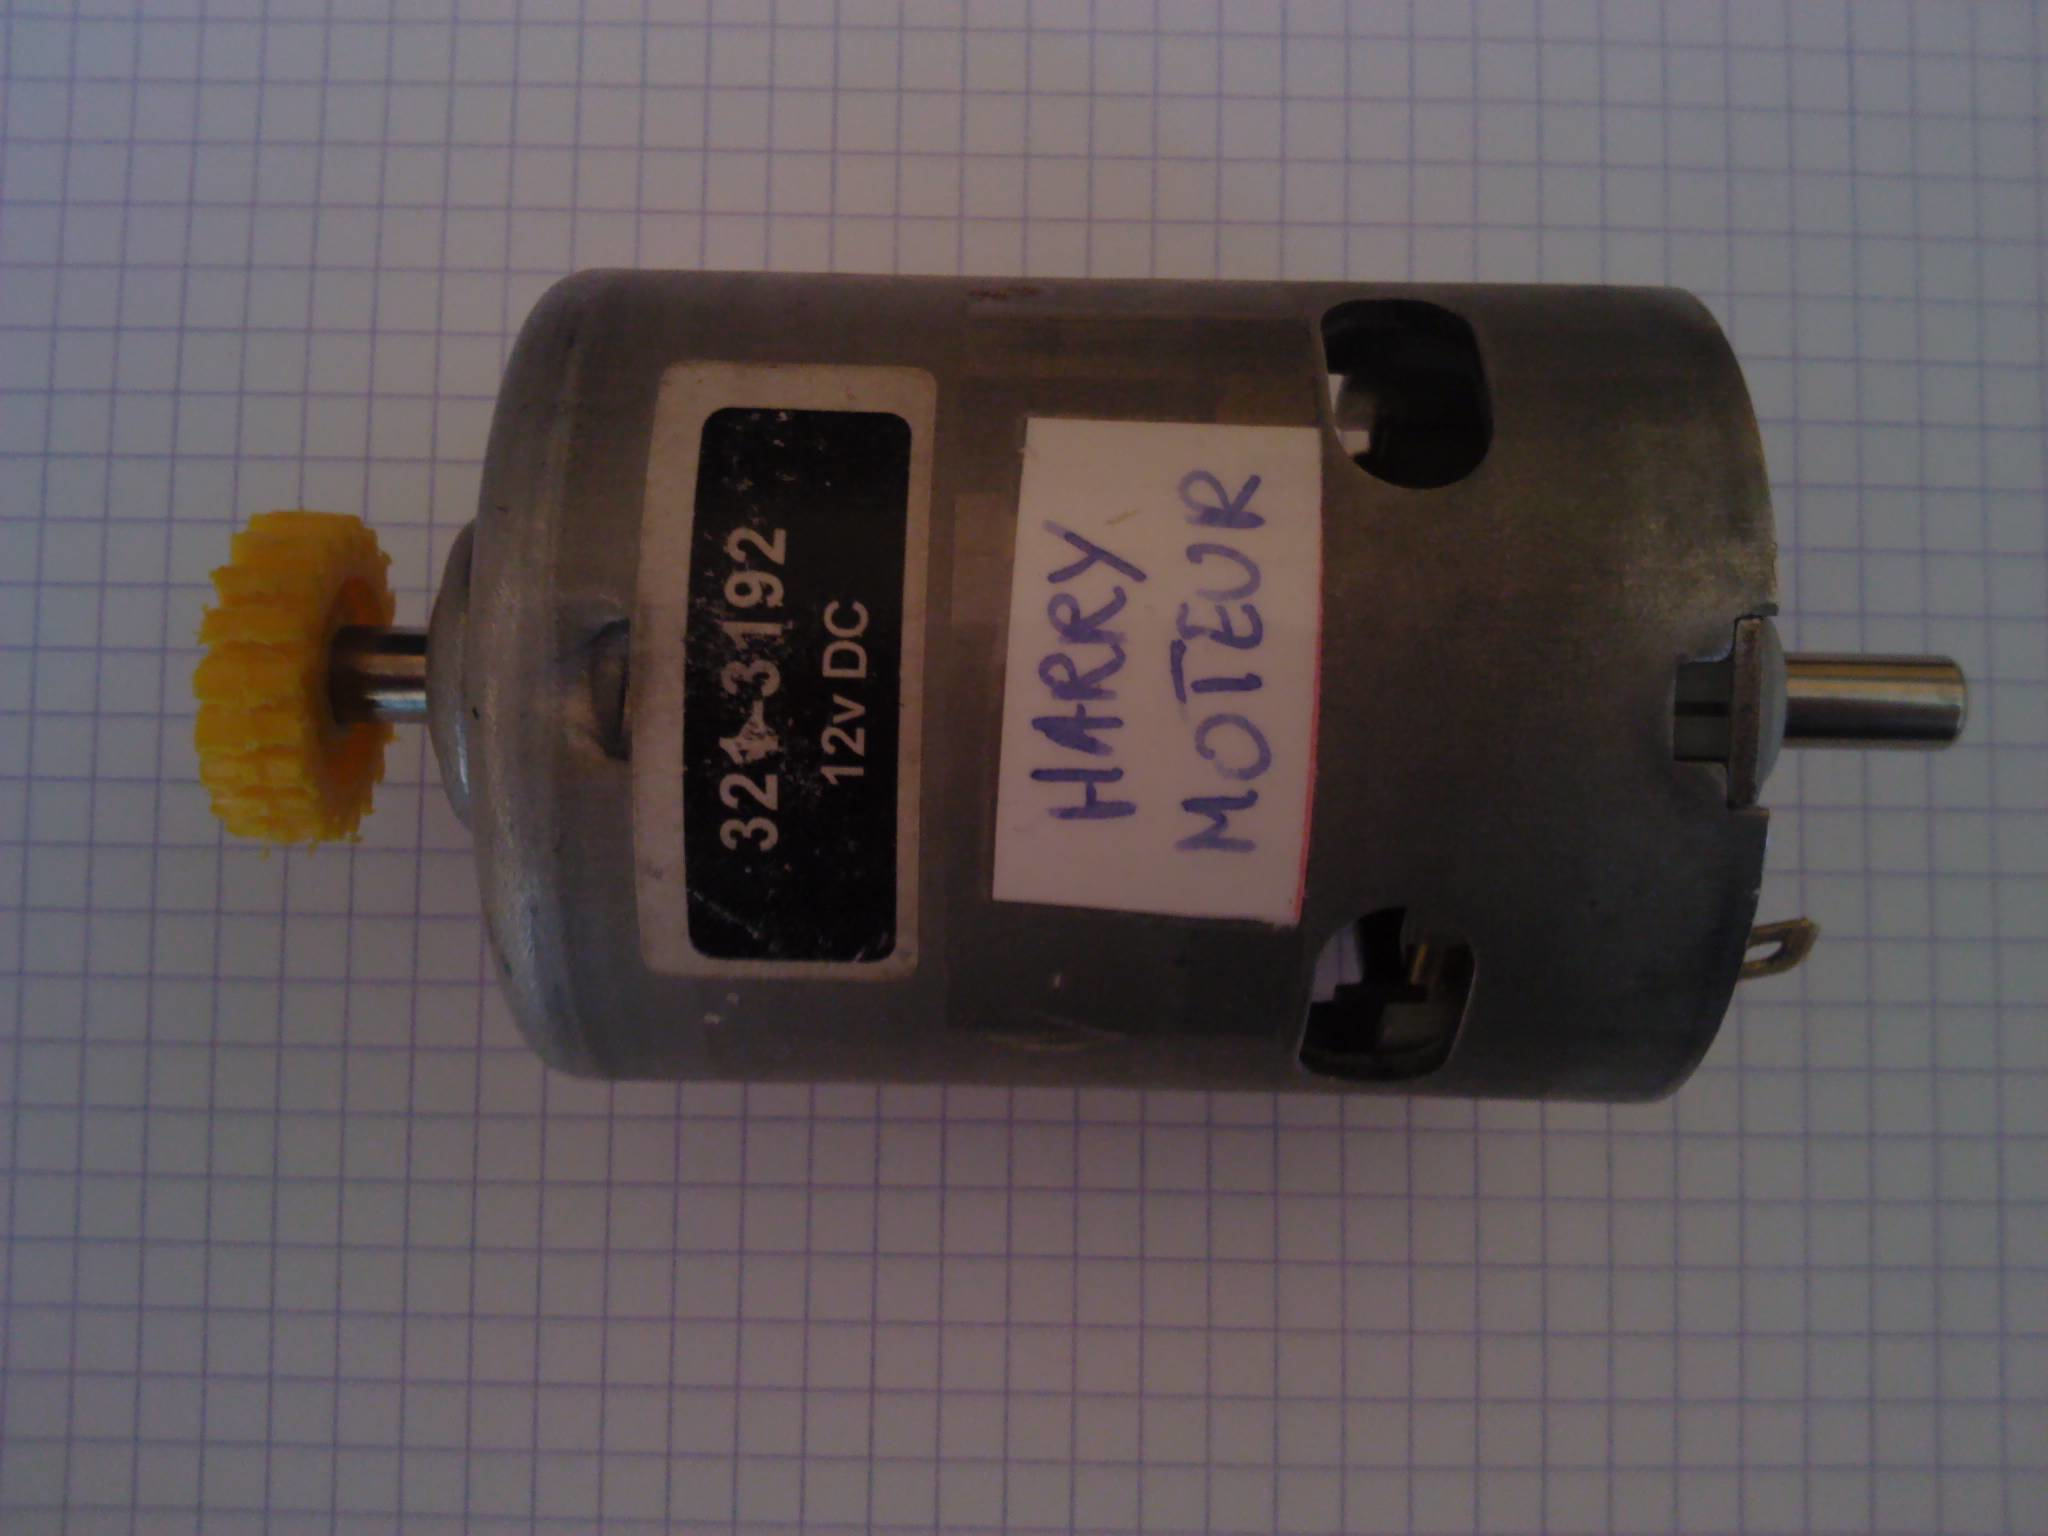
\includegraphics[scale=0.08]{rcs/motor.png}
    \end{center}
    \begin{exampleblock}{Caractéristiques.}
        \[ \omega = 870 rad.s^{-1} \]
        \[ T = 92.13*10^{-3} N.m \]
    \end{exampleblock}
\end{frame}

\begin{frame}
    \frametitle{Réduction.}
    \begin{block}{Facteur.}
        \[ r = \frac{\omega_{entree}}{\omega_{sortie}} \]
        \[ r = 21.75 \]
    \end{block}
    \begin{center}
        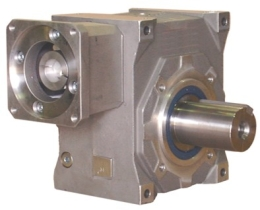
\includegraphics[scale=0.9]{rcs/redu.png}
    \end{center}
\end{frame}

\subsection{Direction.}
\begin{frame}
    \frametitle{Type de direction.}
    \begin{exampleblock}{Avantages.}
        \begin{itemize}
            \item Plus de couple transmis.
            \item Plus de précision.
            \item Plus d'équilibre.
            \item Possibilité de rajouter une suspension.
        \end{itemize}
    \end{exampleblock}
    \only<2-> {
        \begin{alertblock}{Inconvénients.}
            \begin{itemize}
                \item Plus cher.
                \item Plus lourd.
                \item Plus difficile à mettre en œuvre.
            \end{itemize}
        \end{alertblock}
    }
\end{frame}

\begin{frame}
    \frametitle{Simulation.}
    \begin{center}
        \only<1> {
            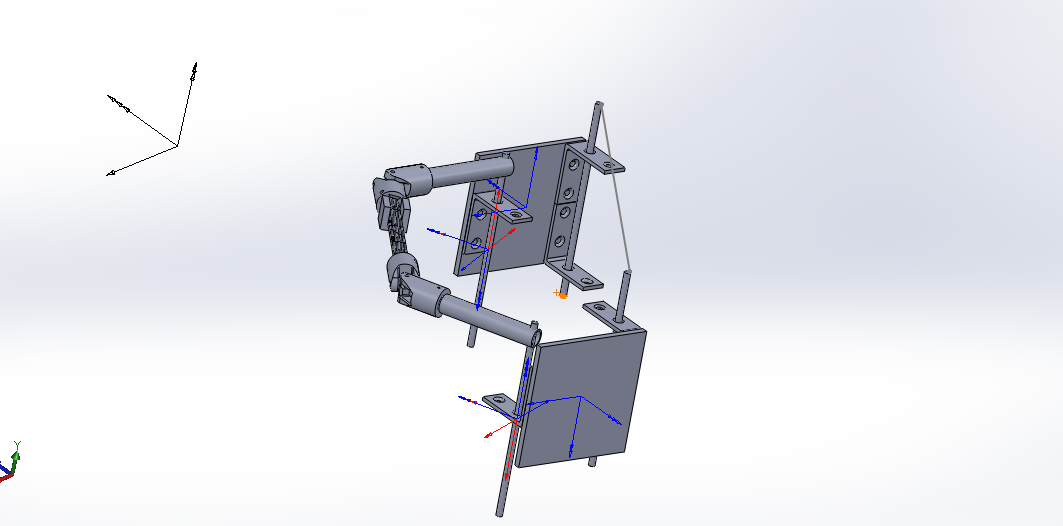
\includegraphics[width=\linewidth]{rcs/solid1.png}
        } \only<2> {
            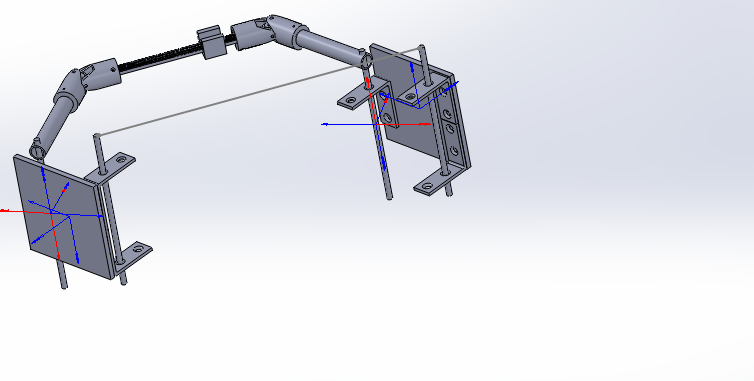
\includegraphics[width=\linewidth]{rcs/solid2.png}
        }
    \end{center}
\end{frame}

\begin{frame}
    \frametitle{Choix du moteur.}
    \begin{block}{Force de guidage.}
        \[ F = \frac{m*v^2}{R} \]
        \[ F = 110 N \]
    \end{block}
    \only<2-> {
        \begin{block}{Rayon de trajectoire.}
            \[ R = \frac{E}{\sin \alpha} \]
            \[ R = 0.85m \]
        \end{block}
    }
    \only<3-> {
        \begin{block}{Puissance.}
            \[ P = F * v \]
            \[ P = 4.40W \]
        \end{block}
    }
\end{frame}


